\section{Approach}
\label{sec:approach}
In this section, we will first introduce the overview of our proposed model and then present each part of the model in detail.

\begin{figure}
	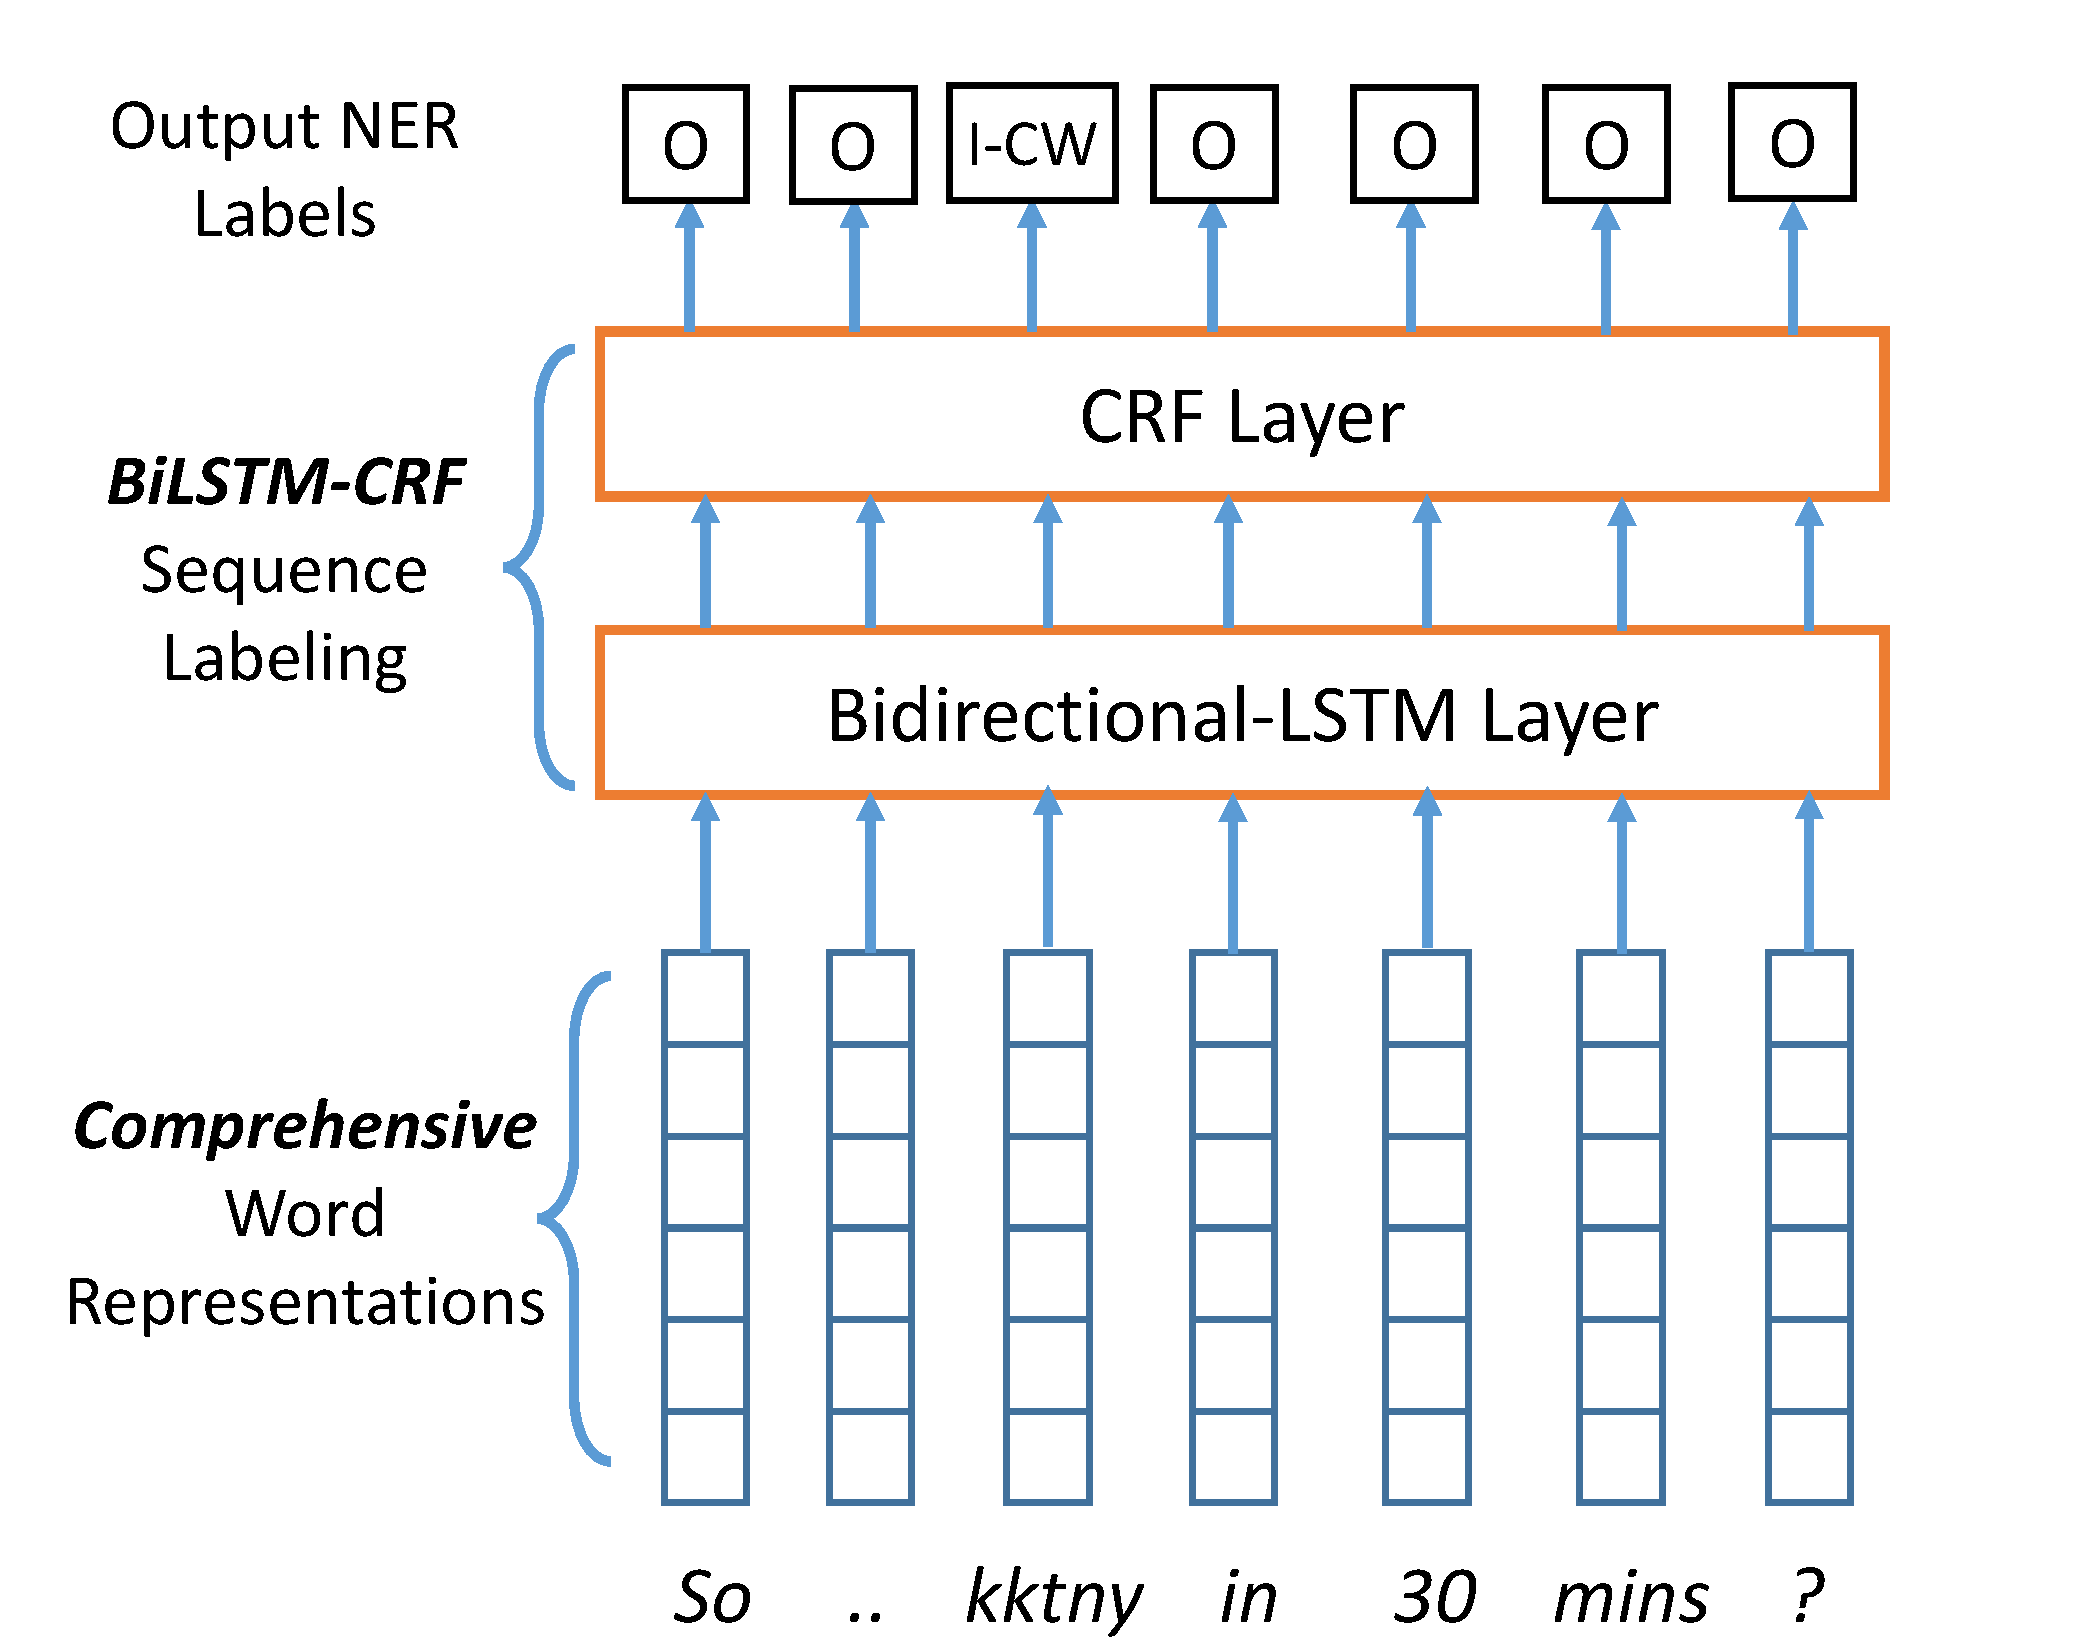
\includegraphics[width=\columnwidth]{figures/overview}
	\caption{Overview of our approach.}
	\label{fig:overall}
\end{figure}

\subsection{Overview}
\figref{fig:overall} shows the overall structure of our proposed model, 
instead of solely using the original pretrained word embeddings as the final word representations, 
we construct a comprehensive word representation for each word in the input sentence.
This comprehensive word representations contain the character-level sub-word information, the original pretrained word embeddings and multiple syntactical features. 
Then, we feed them into a Bidirectional LSTM layer, and thus we have a hidden state for each word. 
The hidden states are considered as the feature vectors of the words by the final CRF layer, from which we can decode the final predicted tag sequence for the input sentence.

\begin{figure}
	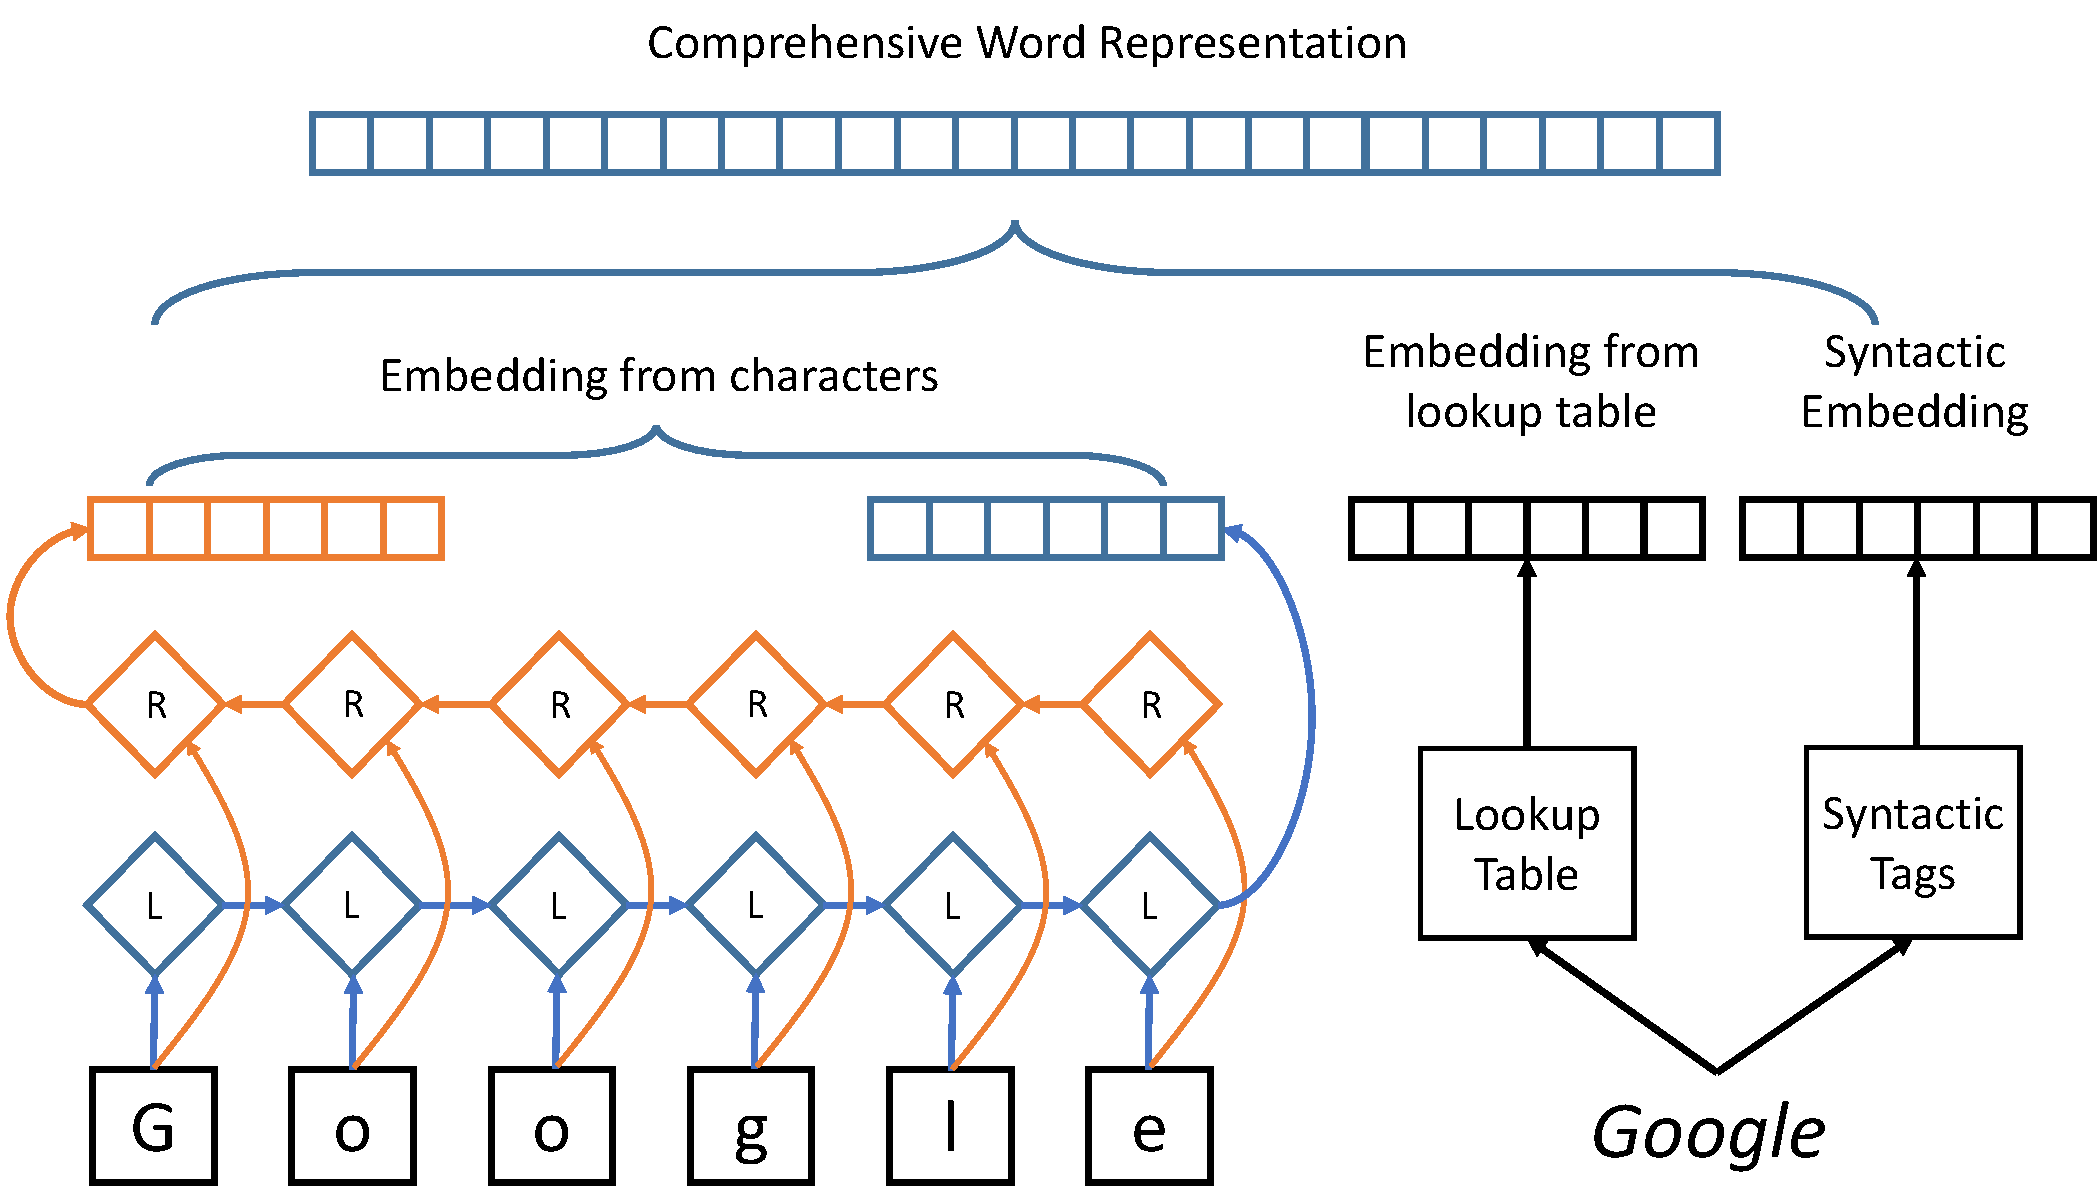
\includegraphics[width=\columnwidth]{figures/comprehensive}
	\caption{Illustration of comprehensive word representation.}
	\label{fig:comprehensive}
\end{figure}

\subsection{Comprehensive Word Representations}
In this subsection, we present our proposed comprehensive word representations. 
We first build character-level word representations from the embeddings of every characters in each word using a bidirectional LSTM. 
Then we further incorporate the final word representation with the embedding of the syntactical information of each token, such as the part-of-speech tag, the dependency role, the position in the sentence and the position of the head. \BL{i am not sure about the HEAD. maybe we can find a better description.}
Finally, we combine the original word embeddings with the above two parts to obtain the final comprehensive word representations.

\subsubsection{Character-level Word Representations}
In noisy user-generated text analysis, sub-word (character-level) information is much more important than that in normal text analysis for two main reasons:
1) People are more likely to use novel abbreviations and morphs to mention entities, which are often out of vocabulary and only occur a few times. 
Thus, solely using the original word-level word embedding as features to represent  words is not adequate to capture the characteristics of such mentions.
2) Another reason why we have to pay more attention to character-level word representation for noisy text is that it is can capture the orthographic or morphological information of both formal words and Internet slang. 

There are two main network structures to make use of character embeddings: 
one is CNN (Ma and Hovy, 2016 \cite{} ) and the other is BiLSTM(Lample et al. 2016).
BiLSTM turns to be better in our experiment on development dataset and we will discuss the reason in \secref{sec:eval}.
Thus, we follow Lample et al. (2016) to build a BiLSTM network to encode the characters in each token as \figref{arg1} shows.
We finally concatenate the forward embedding and backward embedding to the final character-level word representation.

\subsubsection{Syntactical Word Representations}
We argue that the syntactical information, such as POS tag and dependency role, should also be explicitly considered as context features of each token in the sentence. 

Popular opensource software called TweetNLP and TweeboParser~\cite{owoputi2013improved,kong2014dependency} are used to generate such syntactical tags for each token given a tweet.
Given the nature of the noisy tweet text, a new set of POS tags and dependency trees are used in the tool, called Tweebank~\cite{gimpel2011part}. See~\tabref{tbl:pos} for an example POS tagging. Since a tweet often contains more than one utterance, the output of TweeboParser will often be a multi-rooted graph over the tweet.  Head index of the token is taken into account while calculating these embedding vector to further enrich the dependency information. Also, many elements in tweets have no syntactic function. These include, in many cases, hashtags, URLs, and emoticons. It tries to exclude these tokens from the parse tree, resulting a head index of -1.
Position embedding is included as well as it is widely used in other similar tasks, like relation classification~\cite{xu2016improved}.
After calculating all 4 types of embedding vectors (POS, dependency role, position, head) for each token, we concatenate them to form the syntactical word representation.
\begin{table}[]
	\centering
	\caption{Example of POS tagging for tweets.}
	\label{tbl:pos}
	\begin{tabular}{l|c|c|c|c|c|c|c}
		\hline
		Token & so & .. & kktny & in & 30 & mins & ? \\ \hline
		POS   & R  & ,  & N     & P  & \$  & N    & , \\ \hline
		Position & 1&2&3&4&5&6&7\\ \hline
		Head & 0 &-1& 0& 3& 6& 4& -1 \\ \hline
\end{tabular}
\end{table}


\subsubsection{Combination with Word-level Word Representations}
After obtaining the above two additional word representations, we combine them with the original word-level word representations, which are just traditional word embeddings. 

To sum up, our comprehensive word representations are the concatenation of three parts: 1) character-level word representations, 2) syntactical word representation and 3)  original pretrained word embeddings.

\subsection{BiLSTM Layer}
LSTM based networks are proven to be effective in sequence labeling problem for they have access to both past and the future contexts. 
Whereas, hidden states in unidirectional LSTMs only takes information from the past, which may be adequate to classify the sentiment  is a shortcoming for labeling each token.
Bidirectional LSTMs enable the hidden states to capture both historical and future context information and then to label a token.

Mathematically, the input of this BiLSTM layer is a sequence of comprehensive word representations (vectors) for the tokens of the input sentence,  denoted as 
$( \mathbf{x_1}, \mathbf{x_2},...,\mathbf{x_n})$. 
The output of this BiLSTM layer is a sequence of the hidden states for each input word vectors, denoted as 
$( \mathbf{h_1}, \mathbf{h_2},...,\mathbf{h_n})$. 
Each final hidden state is the concatenation of the forward $\overleftarrow{\mathbf{h_i}}$ and backward $\overrightarrow{\mathbf{h_i}}$ hidden states.
We know that 

$$\overleftarrow{\mathbf{h_i}}= \text{lstm}(\mathbf{x_i}, \overleftarrow{\mathbf{h_{i-1}}})~\text{,}~\overrightarrow{\mathbf{h_i}}= \text{lstm}(\mathbf{x_i}, \overrightarrow{\mathbf{h_{i+1}}})$$ 

$$\mathbf{h_i} = \left[~\overleftarrow{\mathbf{h_i}}~;~\overrightarrow{\mathbf{h_i}}~\right]$$


\subsection{CRF Layer}
It is almost always beneficial to consider the correlations between two between current label and neighboring labels since there are many syntactical constrains in natural language sentences. 
For example, I-PERSON will never follow a B-GROUP. 
If we simply feed the above mentioned hidden states independently to a Softmax layer to predict the labels, then such constrains will not be more likely to be broken. 
Linear-chain Conditional Random Field is the most popular way to control the structure prediction and its basic idea is to use a series of potential function to approximate the conditional probability of the output label sequence given the input word sequence. 

Formally, we take the above sequence of hidden states  $ \mathbf{h} = ( \mathbf{h_1}, \mathbf{h_2},...,\mathbf{h_n})$ as our input to the CRF layer, and its output is our final prediction label sequence $\mathbf{y} = ( {y_1}, {y_2},...,{y_n})$, where $y_i$ is in the set of all possible labels. 
We denote $\mathcal{Y}(\mathbf{h})$ as the set of all possible label sequences.
Then we derive the conditional probability of the output sequence given the input hidden state sequence is 

{\scriptsize $$ p(\mathbf{y}|\mathbf{h}; \mathbf{W},\mathbf{b}) 
= \frac{\prod_{i=1}^n \exp(\mathbf{W}^T_{y_{i-1},y_{i}}\mathbf{h} + \mathbf{b}_{y_{i-1},y_{i}})}
{ \sum_{\mathbf{y'} \in \mathcal{Y}(\mathbf{h})} \prod_{i=1}^n \exp(\mathbf{W}^T_{y'_{i-1},y'_{i}}\mathbf{h} + \mathbf{b}_{y'_{i-1},y'_{i}})} 
$$
}

, where $\mathbf W$ and $\mathbf b$ are the two weight matrices and the subscription indicates that we extract the weight vector for the given label pair $(y_{i-1},y_i)$. 

To train the CRF layer, we use the classic maximum conditional likelihood estimation to train our model. 
The final log-likelihood with respect to the weight matrices is 

$$ L(\mathbf{W},\mathbf{b}) = \sum_{(\mathbf{h_i}, \mathbf{y_i})}  \log p(\mathbf{y_i}|\mathbf{h_i}; \mathbf{W},\mathbf{b}) $$
~\\~
Finally, we adopt the Viterbi algorithm for training the CRF layer and the decoding the optimal output sequence $\mathbf{y^*}$.



